\documentclass[a4paper,12pt,french]{book}
\usepackage[margin=2cm]{geometry}
\usepackage[thinfonts]{uglix2}
\nouveaustyle

\begin{document}
\titre{Parcours de graphes}{NSI2}{2022}

\begin{exercice}
On considère le graphe suivant :
\begin{center}
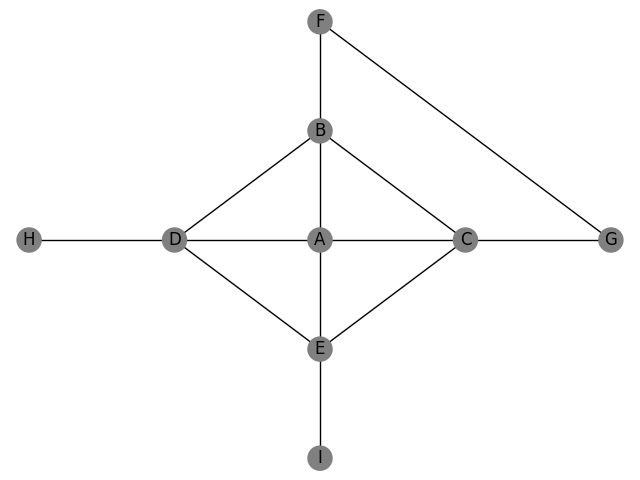
\includegraphics[width=10cm]{img/00.png}
\end{center}
\begin{enumerate}[\bfseries 1.]
	\item On commence par le sommet A.
    \begin{enumerate}[\bfseries a.]
    	\item Réaliser à la main \textit{un} parcours en profondeur du graphe, en indiquant comme dans le cours les états successifs de la pile. Donner à la fin la liste des sommets parcourus. Votre résultat dépendra évidemment de l'ordre dans lequel vous empilez les voisins.\\
        On pourra par exemple choisir de les empiler dans l'ordre alphabétique.
        \item Faire de même dans le cas d'un parcours en largeur, avec une file.
    \end{enumerate}
    \item Recommencer avec le sommet G.
\end{enumerate}
\end{exercice}

\begin{exercice}
Ouvrir le dossier \texttt{scripts} dans \textsc{PyCharm}, et le fichier \texttt{ex2.py}. Compléter la version récursive de DFS.
\end{exercice}

\begin{exercice}
On veut produire une fonction \texttt{dfs\_path} qui
\begin{enumerate}[--]
	\item prend en entrée un graphe \texttt{G} et deux sommets \texttt{start} et \texttt{end};
    \item renvoie la liste des sommets parcourus de \texttt{start} jusqu'à \texttt{end} s'il existe une chaine dont les extrémités sont ces deux sommets;
    \item renvoie la liste vide sinon.
\end{enumerate}
On peut reprendre la fonction \texttt{dfs\_iterative}, enlever la variable \texttt{visited} qui n'a plus d'intérêt et la remplacer par un dictionnaire nommé \texttt{predecessors}, initialisé avec \pythoninline{predecessors[start]=None}.\\
Puis lors du parcours du graphe, si les voisins à ajouter ne sont pas déjà dans ce dictionnaire, on les ajoute en signifiant que leur prédecesseur est le sommet courant.\\
On s'arrête dès que la pile est vide ou que le sommet courant est \texttt{end}.\\
Si le sommet courant est \texttt{end} alors on se sert de \texttt{predecessors} pour reconstruire la liste des sommets partant de \texttt{start} (unique sommet qui a pour prédécesseur \pythoninline{None}) à \texttt{end}.\\
Sinon on renvoie la liste vide.\\

Coder cette fonction.
\end{exercice}

\begin{exercice}
Reprendre l'exercice précédent et coder \pythoninline{bfs_path}.
\end{exercice}
\end{document}